\documentclass{article}
\usepackage[utf8]{inputenc}
\usepackage[hidelinks]{hyperref}
\usepackage[spanish]{babel}
\usepackage[left=2cm,right=2cm,top=2cm,bottom=2cm]{geometry}
\usepackage{graphicx}
\usepackage{pdflscape}
\usepackage{listings}

\lstset {
    frame = single,
    breaklines = true
}


\begin{document}

\begin{titlepage}

\title{\textbf{
    {\Huge Práctica 5: Ejecución de aplicaciones desconocidas/no disponibles}\\
    {\Large Sistemas Legados}
}}
\author{
    Pedro Allué Tamargo (758267)
    \and
    Juan José Tambo Tambo (755742)
    \and
    Jesús Villacampa Sagaste (755739)
}
\date{\today}
\clearpage\maketitle
\thispagestyle{empty}
\tableofcontents
\end{titlepage}

\section{Introducción}

En esta práctica se va a proceder a ejecutar aplicaciones desconocidas de las cuales no se tiene ninguna información. Para esta práctica se han proporcionado dos programas legados. Estos programas se corresponden con un juego y con un sistema de control de inventario.\\
También se debe reproducir una canción en formato \textit{text assist} para las tarjetas de sonido \textit{Sound Blaster}. Este programa no está disponible y habrá que realizar tareas extra para poder conseguir el objetivo.\\


\section{Esfuerzos invertidos}

\begin{itemize}
    \item Pedro Allué Tamargo: Ejecución del \textit{legado1.bin}, \textit{legado2.bin}, modificación del código del \textit{legado2.bin} y apoyo a la recuperación del \textit{software} necesario para reproducir la canción. Memoria de los programas legados.
        \begin{itemize}
            \item Tiempo invertido: 8 horas.
        \end{itemize}
    \item Juan José Tambo Tambo: Ejecución del \textit{legado2.bin} y y apoyo a la recuperación del \textit{software} necesario para reproducir la canción.
        \begin{itemize}
            \item Tiempo invertido: 4 horas.
        \end{itemize}
    \item Jesús Villacampa Sagaste: Ejecución del \textit{legado2.bin}, modificación del código del \textit{legado2.bin}, creación del entorno para reproducir la canción y su posterior grabación. Memoria de la parte de la canción.
        \begin{itemize}
            \item Tiempo invertido: 8 horas.
        \end{itemize}
\end{itemize}


\section{Aplicaciones Legadas}

\subsection{Aplicación \textit{legado1.bin}}

El primer legado se puede abrir con un editor de texto plano y se puede observar la cadena \textit{The Polony David A. Smith} y \textit{1988}. Realizando una búsqueda en Internet se puede observar que se corresponde con el juego \textit{``The Colony''\footnote{\url{https://en.wikipedia.org/wiki/The_Colony_(video_game)}}}. Se corresponde con la captura de pantalla dada en el enunciado.\\
Utilizando el comando \texttt{file legado1.bin} se puede observar la siguiente salida:

\begin{figure}[h!]
    \centering
    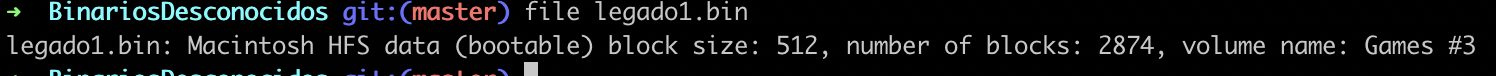
\includegraphics[scale=0.5]{images/file_legado1.png}
    \caption{Captura de pantalla de la salida del comando \texttt{file legado1.bin}}
    \label{fig:fileLegado1}
\end{figure}

Se puede observar que ser corresponde con un fichero de sistema de ficheros de un \textit{Macinstosh}. Por lo tanto el programa legado se corresponde con la versión de \textit{The Colony} para \textit{Macintosh}.\\

Se va a utilizar un emulador \textit{Macintosh} para ejecutar el programa. El emulador utilizado será \textit{mini vMac}. Para la preparación del entorno de emulación se han seguido las indicaciones encontradas en este tutorial\footnote{\url{https://www.emaculation.com/doku.php/mini_vmac_setup}}.\\
Una vez instalado el sistema operativo de \textit{Macintosh} en el emulador se va a proceder a introducir el fichero \textit{legado1.bin}. Para ello se arrastrará el fichero hasta la ventana del emulador. Una vez cargado el sistema de ficheros aparecerá un icono en el escritorio (Figura~\ref{fig:emuladorEscritorio}). Dentro de este sistema de ficheros se puede encontrar el fichero \textit{Colony} (Figura~\ref{fig:emuladorContenidoLegado}). Si lo ejecutamos se cargará el juego y se verá la imagen de la Figura~\ref{fig:emuladorJuego}.\\


\newpage
\subsection{Aplicación \textit{legado2.bin}}

El segundo legado tras abrirlo con un editor de texto plano se puede observar la cadena de texto \textit{ELF} al inicio del fichero. Si se ejecuta el comando \texttt{file legado2.bin} se puede observar la siguiente salida:

\begin{figure}[h!]
    \centering
    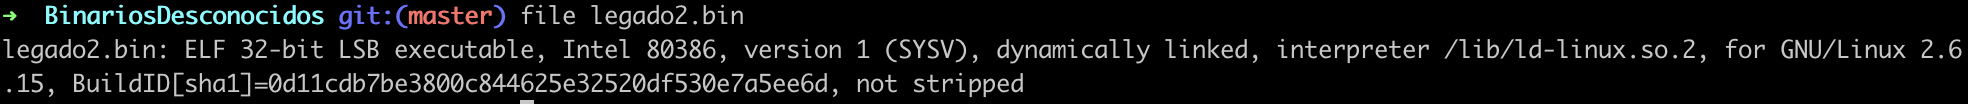
\includegraphics[scale=0.5]{images/file_legado2.png}
    \caption{Captura de pantalla de la salida del comando \texttt{file legado2.bin}}
    \label{fig:fileLegado2}
\end{figure}

Se puede observar que es un binario de 32 bits compilado para el \textit{kernel} de Linux 2.6.15 y para un procesador \textit{Intel 80386}. Al ser de arquitectura x86 se podrá ejecutar sobre un procesador de 64 bits pero se va a utilizar una máquina virtual \textit{Ubuntu 16.04} de 32 bits que es la última que utilizaba el kernel para el que estaba compilada la máquina.\\

Si se inspecciona el fichero se puede observar que se nombra a una llave de protección \textit{Hardware}. Esto significa que el programa tiene una interacción con un elemento \textit{Hardware} externo que impedirá la ejecución del programa con el resultado esperado. Para ejecutar el programa se ha utilizado el comando \texttt{sudo ./legado2.bin}. El resultado de la ejecución puede observarse en la Figura \ref{fig:llaveHW_noEnct}.\\

\begin{figure}[h!]
    \centering
    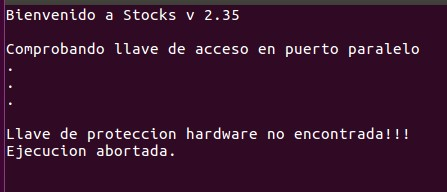
\includegraphics[scale=0.9]{images/llavehw_noenct.jpg}
    \caption{Captura de pantalla de la ejecución de \texttt{legado2.bin} sin modificación de llave hardware}
    \label{fig:llaveHW_noEnct}
\end{figure}\\

Se puede observar que el fichero no se ejecuta correctamente debido a la restricción de la llave de protección \textit{Hardware}. Por lo tanto se va a proceder a modificar el código de la aplicación legada. Para ello se va a utilizar el programa \textit{Ghidra\footnote{\url{https://ghidra-sre.org/}}}. Tras abrir el fichero como parte de un proyecto se va a inspeccionar su código con la opción de `Analizar' que proporciona \textit{Ghidra} y se puede observar su función \texttt{main} (Figura \ref{fig:mainGhDesc}). accediendo a él desde \emph{Symbol Tree -$>$ Functions}.\\

Para modificar el flujo de control del programa se ha modificado la instrucción \texttt{JZ} (Figura \ref{fig:JZ}) que salta a una dirección de memoria (instrucción \texttt{puts("Llave de proteccion encontrada. Ejecucion permitida.");}) si la llave \textit{hardware} se había introducido. Se ha modificado por una instrucción de salto incondicional \texttt{JMP} (Figura \ref{fig:JMP}), por lo que la claúsula \emph{if} de Figura \ref{fig:mainGhDesc} nunca se ejcutará y el código resultante será el de la Figura \ref{fig:mainGh}\\

Por lo tanto, ejecutando el programa sobre la plataforma anterior se obtiene un error de segmentación. Este error se corresponde con un error de la herramienta\footnote{\url{https://reverseengineering.stackexchange.com/questions/25427/segmentation-fault-after-export-binary-file-in-ghidra-even-without-any-changes}}. Para corregir esto se ha utilizado un editor hexadecimal \footnote{\url{https://mh-nexus.de/en/hxd/}} sobre el fichero original. La solución es simple debido a que se conoce el contenido del programa y su codificación en hexadecimal. Se ha buscado la instrucción correspondiente al \textit{JZ} (Figura \ref{fig:hexSinMod}) y se ha modificado por un \textit{JMP} (Figura \ref{fig:hexMod}). Si se ejecuta otra vez el programa legado con el comando \texttt{sudo ./legado2.bin} se obtiene lo mostrado en la Figura \ref{fig:leg2}.\\


\section{Canción del fichero}

Se debe conseguir un archivo en formato \emph{mp3} la canción que se almacena en el fichero proporcionado con la práctica, \emph{cancion.txt}. Este fichero de texto describe una canción en euskera para la aplicación “Text Assist”, incluida en el software distribuido junto a las tarjetas de sonido Creative Sound Blaster 16. \\

Para obtener la información del sistema operativo en el que se puede instalar la tarjeta de sonido Creative Sound Blaster 16 se observa el ejemplo proporcionado en el guión de la práctica y se concluye que es la tarjeta de sonido del sistema operativo \emph{Windows 95}. \\

Para crear una máquina virtual de \emph{Windows 95} se sigue paso a paso el siguiente tutorial: \url{https://www.youtube.com/watch?v=KbLDteibZmA}. En este se crea y configura una máquina Virtual para VirtualBox adecuadamente. Una vez disponible la máquina virtual, se necesita el programa \emph{Text Assist} para reproducir la canción. En el vídeo de ejemplo se puede observar como la tarjeta de sonido es \emph{Sound Blaster AWE64} por lo que se busca en \emph{https://archive.org/details/software} una ISO que correspondan a los drivers de esa tarjeta. Después de varias descargas y pruebas de diferentes ISOs se consigue obtener una ISO que contiene el programa buscado y es la siguiente: \url{https://archive.org/details/soundblasterawe64iso}.\\

Una vez se tiene la \textit{ISO}, se introduce como una unidad óptica en la máquina virtual y se descargan los programas. A continuación, con el programa ya disponible en la máquina (Figura \ref{fig:programas}), se necesita el archivo \emph{cancion.txt} en la máquina virtual. Se ha intentado meterla a la máquina virtual mediante el sistema de carpeta compartida de VirtualBox, pero no ha sido posible. Finalmente se ha optado por crear una \textit{ISO} del archivo \emph{cancion.txt} con el programa \emph{UltraISO}, y que se introduce a la máquina virtual como unidad óptica, donde ya es posible descargarla localmente.\\

Con el programa y la canción, ya es posible reproducirla (Figura \ref{fig:prog_canc}) y modificar la voz y distintos parámetros en función de como se desee que suene. \\

Para grabar la canción en un archivo de extensión \emph{mp3} se conecta un cable \textit{minijack-minijack} a la entrada y a la salida del ordenador, y una vez redirigida la salida (el audio de la canción) a la entrada de audio, se graba con \emph{Audacity} y se obtiene la canción directamente exportada como \emph{mp3} desde el programa.\\


\section{Conclusiones}

Tras la realización de la práctica el equipo de trabajo se ha dado cuenta de la importancia de los emuladores y de preservar el software legado. Gracias al emulador de \textit{Macintosh} se ha podido ejecutar el primer programa legado. El segundo programa legado tenía una contramedida \textit{Hardware} pero gracias a la charla de \textit{Miguel Ángel Horna} (alias \textit{``El Semi''}) se pudo eliminar utilizando una herramienta de desensamblado de código. Con esta herramienta se pudo conseguir alterar el código del segundo programa legado para saltarse la contramedida de la llave \textit{Hardware}.\\
Por último, también es importante preservar el software legado. Gracias a la página de \textit{archive.org\footnote{\url{https://archive.org/}}} se ha podido obtener una copia del \textit{CD} de instalación del \textit{software} necesario para reproducir la canción adjunta al enunciado.\\


\newpage
\section*{Anexo 1: Figuras}

\begin{figure}[h!]
    \centering
    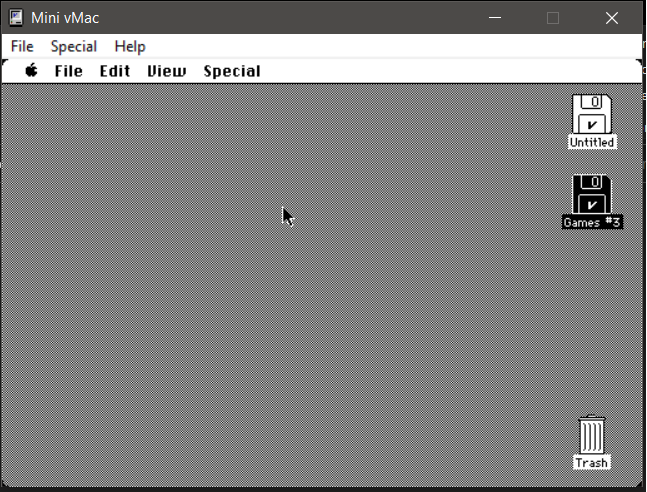
\includegraphics[width=0.8\columnwidth]{images/emuladorEscritorio.png}
    \caption{Captura de pantalla del escritorio del emulador \textit{Mini vMac}}
    \label{fig:emuladorEscritorio}
\end{figure}

\begin{figure}[h!]
    \centering
    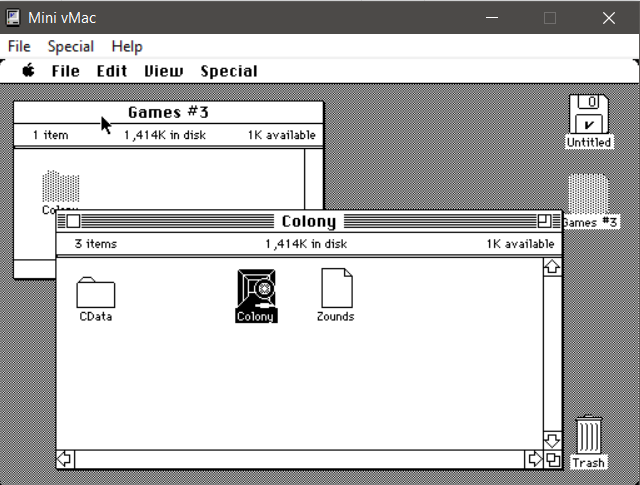
\includegraphics[width=0.8\columnwidth]{images/emuladorSF.png}
    \caption{Captura de pantalla del conetenido de \textit{legado1.bin} en el emulador \textit{Mini vMac}}
    \label{fig:emuladorContenidoLegado}
\end{figure}

\begin{figure}[h!]
    \centering
    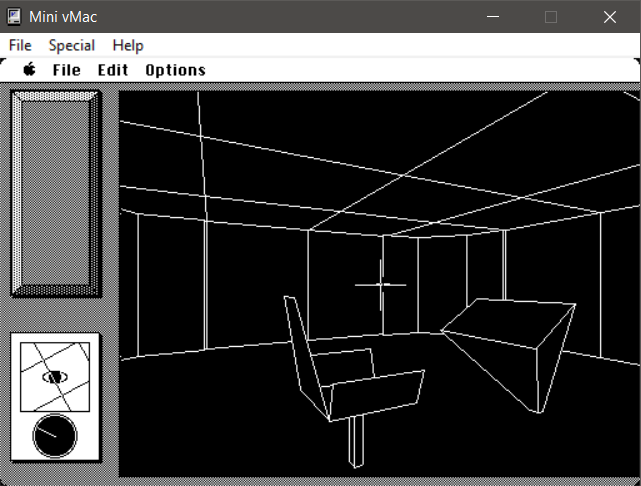
\includegraphics[width=0.8\columnwidth]{images/emuladorJuego.png}
    \caption{Captura de pantalla del juego \textit{legado1.bin} en el emulador \textit{Mini vMac}}
    \label{fig:emuladorJuego}
\end{figure}

\begin{figure}[h!]
    \centering
    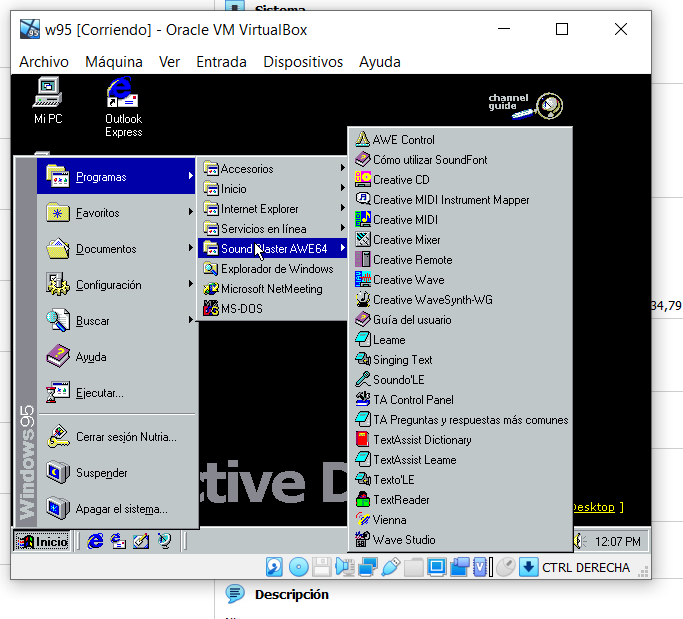
\includegraphics[scale=0.8]{images/programas_SOUNDBLASTER.jpg}
    \caption{Máquina virtual con los programas de Sound Blaster AWE64}
    \label{fig:programas}
\end{figure}

\begin{figure}[h!]
    \centering
    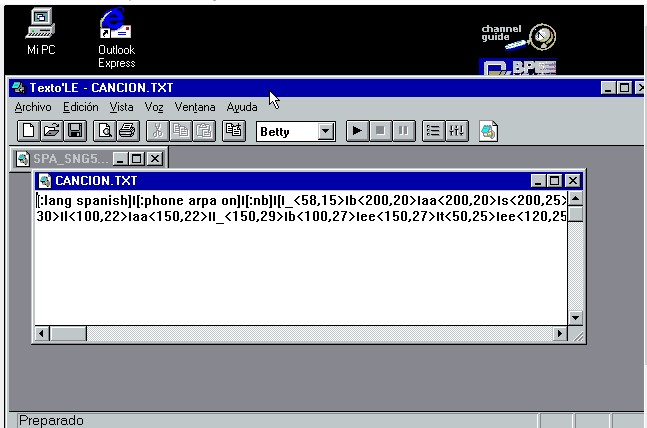
\includegraphics[scale=0.8]{images/textassist_canciontxt.jpg}
    \caption{Canción reproducida por Text Assist}
    \label{fig:prog_canc}
\end{figure}

\begin{figure}[h!]
    \centering
    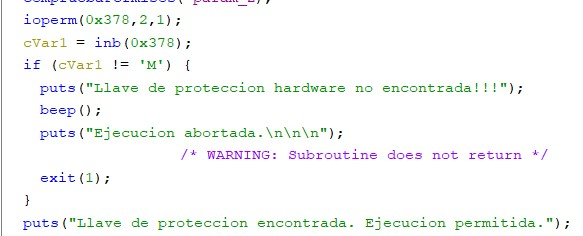
\includegraphics[scale=0.9]{images/mainLeg2Viejo.jpg}
    \caption{Captura de pantalla del main de \texttt{legado2.bin} abierto con \textit{Ghidra}}
    \label{fig:mainGhDesc}
\end{figure}\\

\begin{figure}[h!]
    \centering
    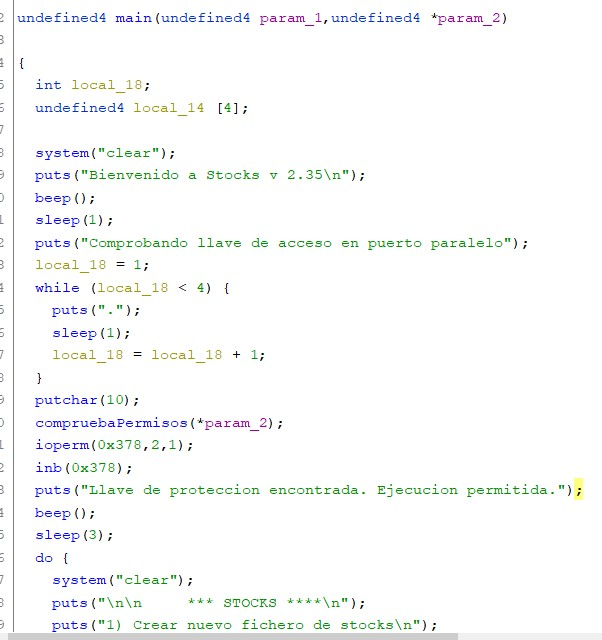
\includegraphics[scale=0.9]{images/mainGhidra.jpg}
    \caption{Captura de pantalla del main de \texttt{legado2.bin} abierto con \textit{Ghidra} sin la comprobación de la llave hardware}
    \label{fig:mainGh}
\end{figure}\\

\begin{figure}[h!]
    \centering
    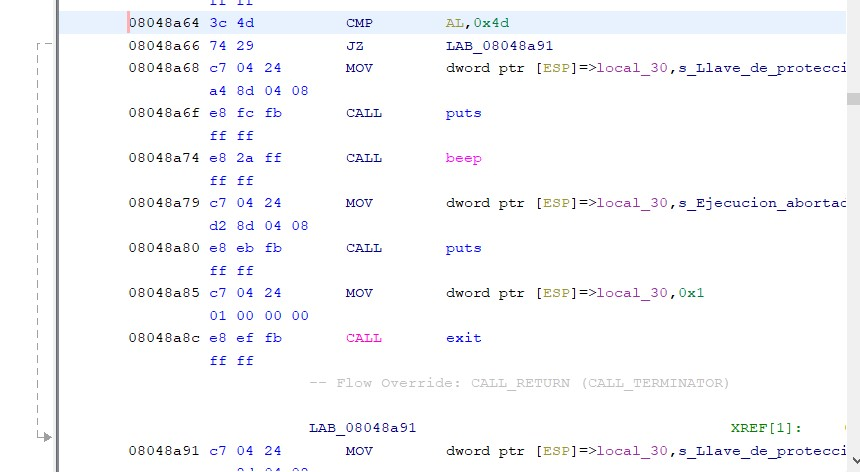
\includegraphics[scale=0.9]{images/codigoMainViejo.jpg}
    \caption{Código del main en ensamblador con la instrucción JZ}
    \label{fig:JZ}
\end{figure}\\

\begin{figure}[h!]
    \centering
    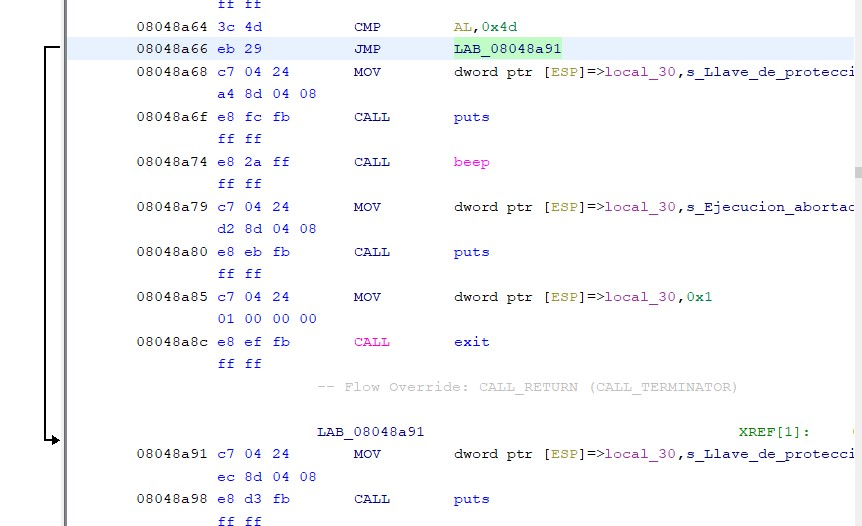
\includegraphics[scale=0.9]{images/cambioLLaveHW.jpg}
    \caption{Código del main en ensamblador con la instrucción JMP}
    \label{fig:JMP}
\end{figure}\\

\begin{figure}[h!]
    \centering
    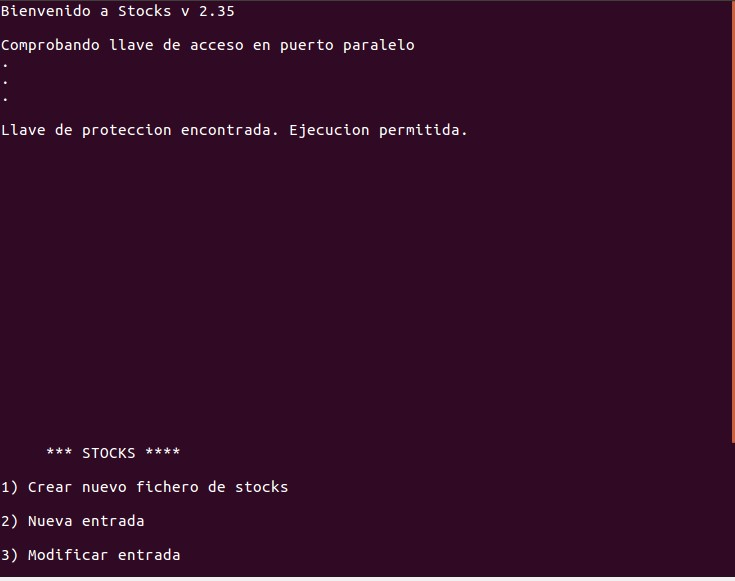
\includegraphics[scale=0.9]{images/appLegado2.jpg}
    \caption{Aplicación \textit{legado2.bin} con el cambio de código de la llave HW}
    \label{fig:leg2}
\end{figure}\\

\begin{figure}[h!]
    \centering
    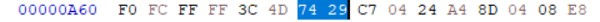
\includegraphics[scale=0.9]{images/hexaSinMod.jpg}
    \caption{Código hexadecimal con intrucción JZ}
    \label{fig:hexSinMod}
\end{figure}\\

\begin{figure}[h!]
    \centering
    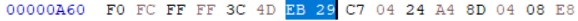
\includegraphics[scale=0.9]{images/hexaMod.jpg}
    \caption{Código hexadecimal con intrucción JMP}
    \label{fig:hexMod}
\end{figure}\\

\end{document}
